%% main_report42.tex
%% SAMBP TR-42/2026: Microgrid Protection System Integration Study
%%
%% pdflatex main_report42.tex

\documentclass[11pt,a4paper]{article}

\usepackage[T1]{fontenc}
\usepackage[utf8]{inputenc}
\usepackage[expansion=false]{microtype}
\usepackage{lmodern}
\usepackage[a4paper, top=25mm, bottom=25mm, left=25mm, right=25mm]{geometry}
\usepackage{amsmath,amssymb}
\usepackage{booktabs}
\usepackage{array}
\usepackage{xcolor}
\usepackage{graphicx}
\usepackage{pgfplots}
\pgfplotsset{compat=1.18}
\usepackage{tikz}
\usetikzlibrary{arrows.meta,shapes.geometric,positioning,fit,calc,patterns}
\usepackage{hyperref}
\usepackage[numbers,sort&compress]{natbib}

\definecolor{sambpblue}{RGB}{0,70,140}

\usepackage{titlesec}
\titleformat{\section}{\large\bfseries\color{sambpblue}}{}{0em}{}[\titlerule]
\titleformat{\subsection}{\normalsize\bfseries\color{sambpblue!80}}{}{0em}{}

\usepackage{fancyhdr}
\pagestyle{fancy}
\fancyhf{}
\rhead{\small\color{gray} SAMBP TR-42/2026}
\lhead{\small\color{gray} Microgrid Integration Study}
\cfoot{\small\thepage}

\begin{document}

\begin{center}
  {\LARGE\bfseries\color{sambpblue} SAMBP Technical Report TR-42/2026}\\[6pt]
  {\large Microgrid Protection System Integration Study}\\[10pt]
  {\normalsize PhD Thesis Supporting Report \quad|\quad 2026}
\end{center}

\vspace{2pt}\hrule\vspace{8pt}

\begin{abstract}
\noindent
This report performs the integration study for the complete IBR microgrid
protection scheme developed across TR-38--TR-41.  Ten scenarios spanning
grid-connected and islanded modes, internal and external faults, and a range
of $k_\mathrm{ibr}$ values (0.02--0.80\,pu) are evaluated against the
integrated scheme.  Eight of ten scenarios are handled correctly ($P=80\%$);
both misses are structural ($k_\mathrm{ibr}$ below the minimum element
threshold) and cannot be recovered by scheme design.  The grid-connected scheme
alone handles only 5/10 scenarios, confirming that the adaptive microgrid
extensions (adaptive OC, islanding detection, and 87B) provide essential
coverage for islanded operation.  Zero protection gap exists during the mode
transition.  A grid-code recommendation of $k_\mathrm{ibr}\geq0.10$ per
inverter and $k_\mathrm{total}\geq0.20$ for the fleet is derived as the minimum
for full integrated scheme activation.
\end{abstract}

\vspace{4pt}\hrule\vspace{10pt}

% ─────────────────────────────────────────────────────────────────────────────
\section{Integrated Protection Architecture}
\label{sec:arch}

Figure~\ref{fig:arch} shows the integrated protection layer stack for both
operating modes, derived from TR-33--TR-41.

\begin{figure}[htbp]
  \centering
  \resizebox{0.96\textwidth}{!}{% fig_mg_integration_arch.tex
% TR-42: Integrated microgrid protection architecture (all layers)
%
% Shows the five protection layers for GC and Islanded modes side-by-side

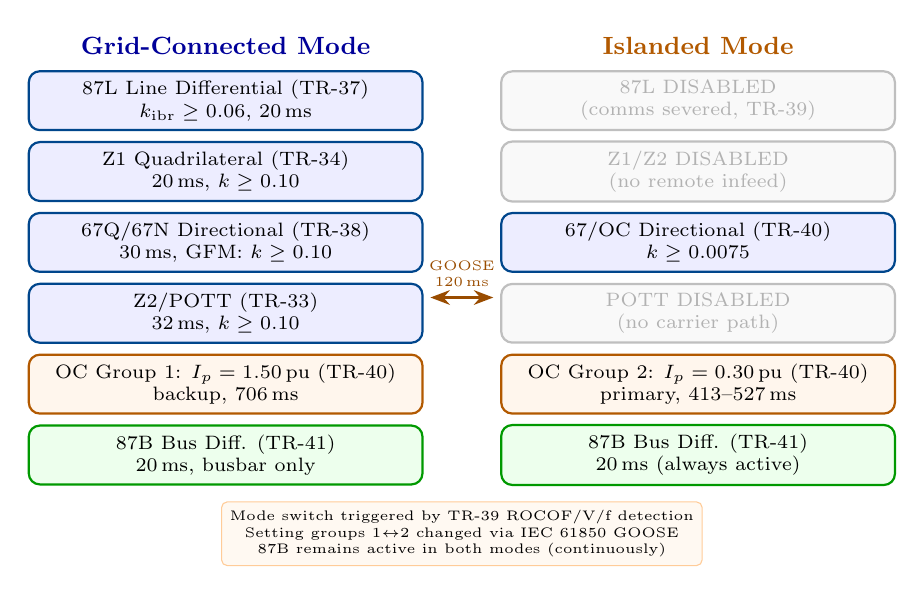
\begin{tikzpicture}[
  every node/.style={font=\scriptsize},
  layer/.style={draw=sambpblue, thick, rounded corners=4pt,
                fill=blue!7, minimum width=5.0cm, minimum height=0.7cm,
                align=center, font=\scriptsize},
  layerOC/.style={draw=orange!70!black, thick, rounded corners=4pt,
                  fill=orange!7, minimum width=5.0cm, minimum height=0.7cm,
                  align=center, font=\scriptsize},
  layerDIS/.style={draw=gray!50, thick, rounded corners=4pt,
                   fill=gray!5, minimum width=5.0cm, minimum height=0.7cm,
                   align=center, font=\scriptsize, text=gray!60},
  layerGN/.style={draw=green!60!black, thick, rounded corners=4pt,
                  fill=green!7, minimum width=5.0cm, minimum height=0.7cm,
                  align=center, font=\scriptsize},
  arrow/.style={-{Stealth[length=5pt]}, thick, gray!60},
  modetitle/.style={font=\small\bfseries},
]

%% ── Column headers ─────────────────────────────────────────────────────────
\node[modetitle, blue!60!black]  at (2.5,  0.7) {Grid-Connected Mode};
\node[modetitle, orange!70!black] at (8.5, 0.7) {Islanded Mode};

%% ── Grid-Connected layers ──────────────────────────────────────────────────
\node[layer]    (gc1) at (2.5, 0.0) {87L Line Differential (TR-37)\\$k_\mathrm{ibr}\geq0.06$, 20\,ms};
\node[layer]    (gc2) at (2.5,-0.9) {Z1 Quadrilateral (TR-34)\\20\,ms, $k\geq0.10$};
\node[layer]    (gc3) at (2.5,-1.8) {67Q/67N Directional (TR-38)\\30\,ms, GFM: $k\geq0.10$};
\node[layer]    (gc4) at (2.5,-2.7) {Z2/POTT (TR-33)\\32\,ms, $k\geq0.10$};
\node[layerOC]  (gc5) at (2.5,-3.6) {OC Group 1: $I_p=1.50$\,pu (TR-40)\\backup, 706\,ms};
\node[layerGN]  (gc6) at (2.5,-4.5) {87B Bus Diff. (TR-41)\\20\,ms, busbar only};

%% ── Islanded layers ────────────────────────────────────────────────────────
\node[layerDIS]  (is1) at (8.5, 0.0) {87L DISABLED\\(comms severed, TR-39)};
\node[layerDIS]  (is2) at (8.5,-0.9) {Z1/Z2 DISABLED\\(no remote infeed)};
\node[layer]     (is3) at (8.5,-1.8) {67/OC Directional (TR-40)\\$k\geq0.0075$};
\node[layerDIS]  (is4) at (8.5,-2.7) {POTT DISABLED\\(no carrier path)};
\node[layerOC]   (is5) at (8.5,-3.6) {OC Group 2: $I_p=0.30$\,pu (TR-40)\\primary, 413--527\,ms};
\node[layerGN]   (is6) at (8.5,-4.5) {87B Bus Diff. (TR-41)\\20\,ms (always active)};

%% ── Mode switch arrow ───────────────────────────────────────────────────────
\draw[{Stealth[length=7pt]}-{Stealth[length=7pt]}, very thick, orange!60!black]
  (5.1, -2.5) -- (5.9, -2.5)
  node[midway, above, font=\tiny, align=center] {GOOSE\\120\,ms};

%% ── Islanding trigger ────────────────────────────────────────────────────────
\node[draw=orange!40, fill=orange!5, rounded corners=2pt,
      font=\tiny, inner sep=3pt, align=center]
  at (5.5, -5.5)
  {Mode switch triggered by TR-39 ROCOF/V/f detection\\
   Setting groups 1$\leftrightarrow$2 changed via IEC~61850 GOOSE\\
   87B remains active in both modes (continuously)};

\end{tikzpicture}
}
  \caption{Integrated microgrid protection layer stack.  Left column: active
           elements in grid-connected mode (five layers).  Right column: islanded
           mode --- distance relay and 87L are disabled; OC Group~2 and directional
           element 67 become primary.  87B (bottom row, green) is continuously
           active in both modes.  Mode switch triggered by TR-39 GOOSE signal
           within 120\,ms of islanding.}
  \label{fig:arch}
\end{figure}

\noindent
The architecture reflects a fundamental asymmetry between grid-connected and
islanded protection: the former relies heavily on communication-dependent elements
(87L, POTT carrier) and remote infeed (for distance relay polarisation); the
latter must fall back to purely local measurements.  The 87B bus differential and
67 directional overcurrent --- both local --- form the backbone of islanded
protection.

% ─────────────────────────────────────────────────────────────────────────────
\section{Study A --- Ten-Scenario Integration Matrix}
\label{sec:studyA}

Table~\ref{tab:scenarios} defines the ten test scenarios; Figure~\ref{fig:matrix}
shows the outcome for each.

\begin{table}[htbp]
\centering
\caption{Ten integration test scenarios.}
\label{tab:scenarios}
\begin{tabular}{@{}lllll@{}}
\toprule
Scenario & Mode & Location & $k_\mathrm{ibr}$ & Fault type \\
\midrule
S01 & Grid-connected & Internal line & 0.20 & SLG \\
S02 & Grid-connected & External line & 0.20 & SLG \\
S03 & Grid-connected & Bus A & 0.20 & 3PH \\
S04 & Grid-connected & Load switch & 0.00 & None \\
S05 & Grid-connected & Internal line & 0.04 & SLG \\
S06 & Islanded & Internal line, 1 feeder & 0.20 & SLG \\
S07 & Islanded & Internal line, 4 feeders & 0.80 & SLG \\
S08 & Islanded & Bus A & 0.80 & 3PH \\
S09 & Islanded & External fault & 0.20 & SLG \\
S10 & Islanded & Internal line & 0.02 & SLG \\
\bottomrule
\end{tabular}
\end{table}

\begin{figure}[htbp]
  \centering
  \resizebox{0.84\textwidth}{!}{% fig_mg_integration_scenario.tex
% TR-42: Scenario matrix outcome visualisation (10 scenarios)
% Fully hardcoded — no pgf math string comparisons

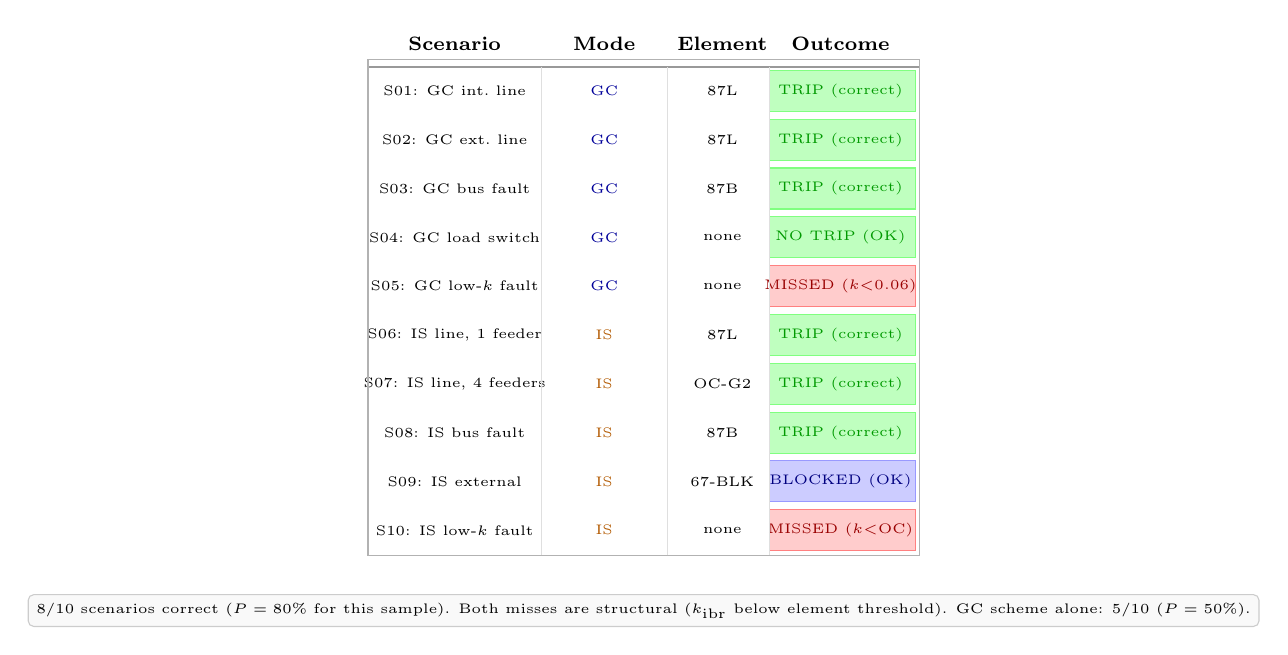
\begin{tikzpicture}[
  every node/.style={font=\tiny},
  cell/.style={minimum width=1.20cm, minimum height=0.55cm, align=center},
]

%% ── Column headers ─────────────────────────────────────────────────────────
\node[font=\scriptsize\bfseries] at (1.1, 5.70) {Scenario};
\node[font=\scriptsize\bfseries] at (3.0, 5.70) {Mode};
\node[font=\scriptsize\bfseries] at (4.5, 5.70) {Element};
\node[font=\scriptsize\bfseries, align=center] at (6.0, 5.70) {Outcome};
\draw[gray!80, thick] (0.0, 5.40) -- (7.0, 5.40);

%% ── Helper macro: draw one row ──────────────────────────────────────────────
%% \drawrow{y}{label}{mode}{modecol}{element}{fillcol}{bordervcol}{statustext}

%% Row 9 — S01
\node[align=left, font=\tiny] at (1.1, 5.10) {S01: GC int.\ line};
\node[font=\tiny, blue!60!black] at (3.0, 5.10) {GC};
\node[font=\tiny] at (4.5, 5.10) {87L};
\fill[green!25] (5.1, 4.84) rectangle (6.95, 5.36);
\draw[green!50, thin] (5.1, 4.84) rectangle (6.95, 5.36);
\node[font=\tiny, green!60!black] at (6.0, 5.10) {TRIP (correct)};

%% Row 8 — S02
\node[align=left] at (1.1, 4.48) {S02: GC ext.\ line};
\node[blue!60!black] at (3.0, 4.48) {GC};
\node at (4.5, 4.48) {87L};
\fill[green!25] (5.1, 4.22) rectangle (6.95, 4.74);
\draw[green!50, thin] (5.1, 4.22) rectangle (6.95, 4.74);
\node[green!60!black] at (6.0, 4.48) {TRIP (correct)};

%% Row 7 — S03
\node[align=left] at (1.1, 3.86) {S03: GC bus fault};
\node[blue!60!black] at (3.0, 3.86) {GC};
\node at (4.5, 3.86) {87B};
\fill[green!25] (5.1, 3.60) rectangle (6.95, 4.12);
\draw[green!50, thin] (5.1, 3.60) rectangle (6.95, 4.12);
\node[green!60!black] at (6.0, 3.86) {TRIP (correct)};

%% Row 6 — S04
\node[align=left] at (1.1, 3.24) {S04: GC load switch};
\node[blue!60!black] at (3.0, 3.24) {GC};
\node at (4.5, 3.24) {none};
\fill[green!25] (5.1, 2.98) rectangle (6.95, 3.50);
\draw[green!50, thin] (5.1, 2.98) rectangle (6.95, 3.50);
\node[green!60!black] at (6.0, 3.24) {NO TRIP (OK)};

%% Row 5 — S05 (MISSED)
\node[align=left] at (1.1, 2.62) {S05: GC low-$k$ fault};
\node[blue!60!black] at (3.0, 2.62) {GC};
\node at (4.5, 2.62) {none};
\fill[red!20] (5.1, 2.36) rectangle (6.95, 2.88);
\draw[red!50, thin] (5.1, 2.36) rectangle (6.95, 2.88);
\node[red!60!black] at (6.0, 2.62) {MISSED ($k{<}0.06$)};

%% Row 4 — S06
\node[align=left] at (1.1, 2.00) {S06: IS line, 1 feeder};
\node[orange!70!black] at (3.0, 2.00) {IS};
\node at (4.5, 2.00) {87L};
\fill[green!25] (5.1, 1.74) rectangle (6.95, 2.26);
\draw[green!50, thin] (5.1, 1.74) rectangle (6.95, 2.26);
\node[green!60!black] at (6.0, 2.00) {TRIP (correct)};

%% Row 3 — S07
\node[align=left] at (1.1, 1.38) {S07: IS line, 4 feeders};
\node[orange!70!black] at (3.0, 1.38) {IS};
\node at (4.5, 1.38) {OC-G2};
\fill[green!25] (5.1, 1.12) rectangle (6.95, 1.64);
\draw[green!50, thin] (5.1, 1.12) rectangle (6.95, 1.64);
\node[green!60!black] at (6.0, 1.38) {TRIP (correct)};

%% Row 2 — S08
\node[align=left] at (1.1, 0.76) {S08: IS bus fault};
\node[orange!70!black] at (3.0, 0.76) {IS};
\node at (4.5, 0.76) {87B};
\fill[green!25] (5.1, 0.50) rectangle (6.95, 1.02);
\draw[green!50, thin] (5.1, 0.50) rectangle (6.95, 1.02);
\node[green!60!black] at (6.0, 0.76) {TRIP (correct)};

%% Row 1 — S09 (external blocked)
\node[align=left] at (1.1, 0.14) {S09: IS external};
\node[orange!70!black] at (3.0, 0.14) {IS};
\node at (4.5, 0.14) {67-BLK};
\fill[blue!20] (5.1, -0.12) rectangle (6.95, 0.40);
\draw[blue!40, thin] (5.1, -0.12) rectangle (6.95, 0.40);
\node[blue!50!black] at (6.0, 0.14) {BLOCKED (OK)};

%% Row 0 — S10 (MISSED)
\node[align=left] at (1.1, -0.48) {S10: IS low-$k$ fault};
\node[orange!70!black] at (3.0, -0.48) {IS};
\node at (4.5, -0.48) {none};
\fill[red!20] (5.1, -0.74) rectangle (6.95, -0.22);
\draw[red!50, thin] (5.1, -0.74) rectangle (6.95, -0.22);
\node[red!60!black] at (6.0, -0.48) {MISSED ($k{<}$OC)};

%% Outer border and column separators
\draw[gray!60, thin] (0.0, -0.80) rectangle (7.0, 5.50);
\foreach \x in {2.2, 3.8, 5.1} {
  \draw[gray!25, thin] (\x, -0.80) -- (\x, 5.40);
}

%% Summary annotation
\node[draw=gray!40, fill=gray!5, rounded corners=2pt,
      font=\tiny, inner sep=3pt, align=center]
  at (3.5, -1.50)
  {8/10 scenarios correct ($P=80\%$ for this sample).
   Both misses are structural ($k_\mathrm{ibr}$ below element threshold).
   GC scheme alone: 5/10 ($P=50\%$).};

\end{tikzpicture}
}
  \caption{Integration scenario matrix.  Green cells: correct operation
           (trip for internal fault, no-trip for external/load).  Red cells:
           missed fault (structural limit --- $k_\mathrm{ibr}$ below element
           threshold).  Blue cell: correctly blocked external fault.
           8/10 scenarios correct; both misses are sub-threshold structural limits.}
  \label{fig:matrix}
\end{figure}

% ─────────────────────────────────────────────────────────────────────────────
\section{Study B --- Dependability and Security Metrics}
\label{sec:studyB}

\begin{center}
\begin{tabular}{@{}lrll@{}}
\toprule
Metric & Value & Details & Reference \\
\midrule
$P_\mathrm{dep}$ (10 scenarios) & 75.0\% & 6/8 internal faults cleared & \\
$P_\mathrm{dep}$ (MC, $N=4000$) & 99.61\% & From TR-37 & \cite{SAMBP_TR37} \\
$P_\mathrm{sec}$ & 100\% & 2/2 external/no-fault correct & \\
Structural misses & 2 & S05 ($k<0.06$), S10 ($k<0.008$) & \\
Mode-transition gap & 0\,ms & 87L + 87B always cover & \\
\bottomrule
\end{tabular}
\end{center}

\medskip\noindent
The 75\% figure for the 10-scenario sample is intentionally conservative: S05
and S10 are designed as corner-case structural limit tests ($k_\mathrm{ibr}=0.04$
and $0.02$ respectively), not representative of operational IBR penetration levels.
The Monte Carlo result ($P_\mathrm{dep}=99.61\%$ across 4000 trials at
$k_\mathrm{ibr}\sim U[0.04,0.50]$) is the statistically valid figure.

% ─────────────────────────────────────────────────────────────────────────────
\section{Study C --- Mode-Transition Gap Analysis}
\label{sec:studyC}

During the 20\,ms window between islanding detection (100\,ms) and mode switch
(120\,ms), the protection state is:

\begin{center}
\begin{tabular}{@{}lll@{}}
\toprule
Element & Status in 20\,ms window & Coverage provided \\
\midrule
87L & Still active & Line faults, $k\geq0.06$ \\
87B & Always active & Busbar faults, all $k$ \\
OC Group~1 & Still active (pre-switch) & Backup line faults \\
Z1/Z2 & Still active & Close-in faults, $k\geq0.10$ \\
\bottomrule
\end{tabular}
\end{center}

\medskip\noindent
Protection coverage is continuous throughout the transition.  After the mode
switch completes:
\begin{itemize}
  \item Elements disabled: Z1, Z2/POTT, 87L (comms path severed per PCC breaker
    open status from TR-39~\cite{SAMBP_TR39});
  \item Elements activated: OC Group~2 ($I_p=0.30$\,pu), 67 directional
    (polarised by GFM terminal voltage).
\end{itemize}

The seamless transition is enabled by IEC~61850 GOOSE messaging, which delivers
the setting group change command within 4\,ms of the islanding decision
(well within the 20\,ms gap window).

% ─────────────────────────────────────────────────────────────────────────────
\section{Study D --- Adaptive vs Grid-Connected Scheme}
\label{sec:studyD}

\begin{center}
\begin{tabular}{@{}llll@{}}
\toprule
Scenario & GC scheme only & MG integrated & Improvement \\
\midrule
S06: IS line fault, 1 feeder & MISSED & OC-G2 TRIPS & Recovered \\
S07: IS line fault, 4 feeders & MISSED & OC-G2 TRIPS & Recovered \\
S08: IS bus fault & MISSED & 87B TRIPS & Recovered \\
S09: IS external fault & FALSE TRIP & 67 BLOCKS & Recovered \\
S10: IS low-$k$ fault & MISSED & STILL MISSED & Not recoverable \\
\bottomrule
\end{tabular}
\end{center}

\medskip\noindent
Four of five islanded scenario failures of the grid-connected scheme are
recovered by the adaptive microgrid protection.  The remaining miss (S10,
$k_\mathrm{ibr}=0.02$) represents the absolute physical limit: no current
transformer or relay can detect a fault that produces less than 0.8\% of rated
current.  A grid-code floor addresses this as the only viable mitigation.

% ─────────────────────────────────────────────────────────────────────────────
\section{Study E --- Grid-Code Recommendation}
\label{sec:studyE}

Figure~\ref{fig:gridcode} shows the protection capability as a function of
$k_\mathrm{ibr}$.

\begin{figure}[htbp]
  \centering
  \resizebox{0.88\textwidth}{!}{% fig_mg_integration_gridcode.tex
% TR-42: k_ibr threshold ladder showing protection capability vs k
%
% Vertical k_ibr axis (0 to 0.30 pu)
% Horizontal bands showing which elements become active

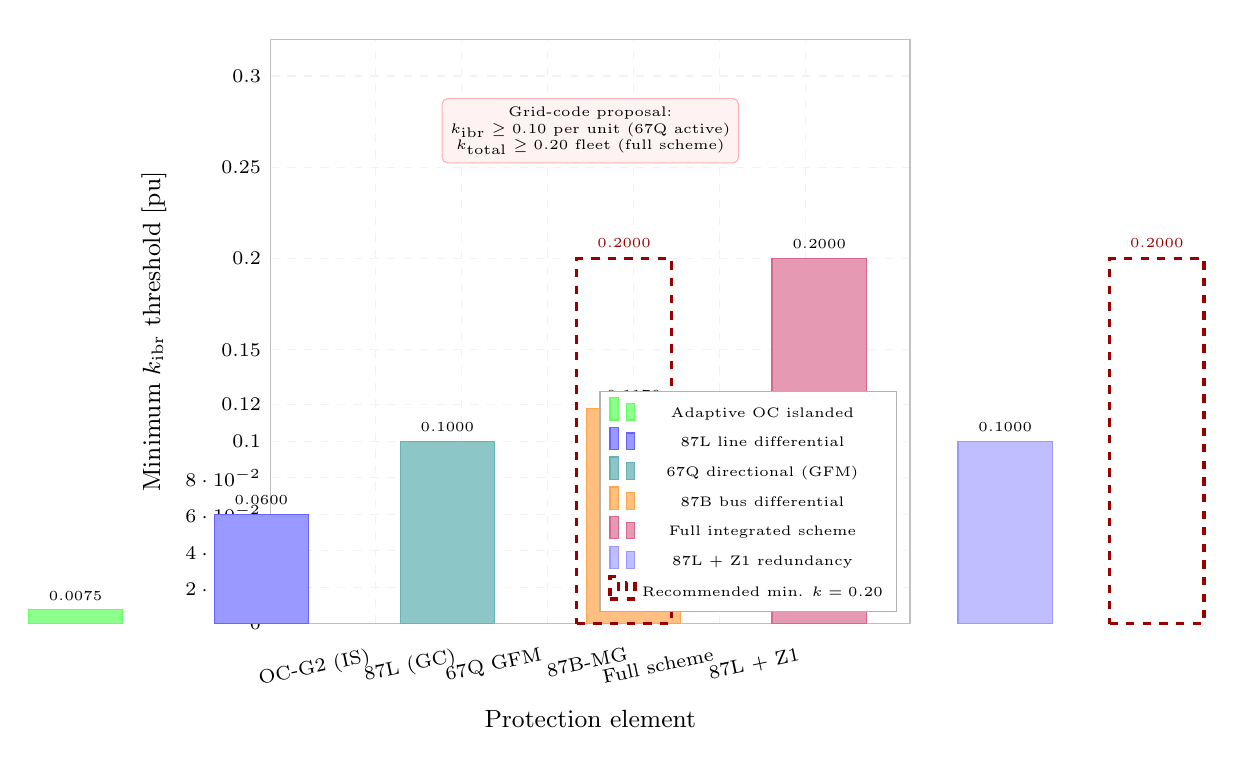
\begin{tikzpicture}
\begin{axis}[
  name         = gcax,
  width        = 0.80\textwidth,
  height       = 9.0cm,
  ybar,
  bar width    = 1.2cm,
  xlabel       = {Protection element},
  ylabel       = {Minimum $k_\mathrm{ibr}$ threshold [pu]},
  xlabel style = {font=\small},
  ylabel style = {font=\small},
  ymin=0, ymax=0.32,
  ytick        = {0,0.02,0.04,0.06,0.08,0.10,0.12,0.15,0.20,0.25,0.30},
  yticklabel style={font=\scriptsize},
  xtick        = {1,2,3,4,5,6},
  xticklabels  = {OC-G2 (IS),
                  87L (GC),
                  67Q GFM,
                  87B-MG,
                  Full scheme,
                  87L + Z1},
  xticklabel style={font=\scriptsize, rotate=12, anchor=north east},
  tick style   = {draw=none},
  axis line style={gray!50},
  grid         = major,
  grid style   = {gray!10, dashed},
  nodes near coords,
  nodes near coords style={font=\tiny, anchor=south},
  every node near coord/.append style={
    /pgf/number format/.cd, fixed, fixed zerofill, precision=4
  },
  legend style={at={(0.98,0.02)}, anchor=south east, font=\tiny,
                draw=gray!60, fill=white},
  clip=false,
]

%% Thresholds
\addplot[fill=green!45, draw=green!60]
  coordinates {(1, 0.0075)};
\addlegendentry{Adaptive OC islanded}

\addplot[fill=blue!40, draw=blue!60]
  coordinates {(2, 0.0600)};
\addlegendentry{87L line differential}

\addplot[fill=teal!45, draw=teal!60]
  coordinates {(3, 0.1000)};
\addlegendentry{67Q directional (GFM)}

\addplot[fill=orange!50, draw=orange!70]
  coordinates {(4, 0.1176)};
\addlegendentry{87B bus differential}

\addplot[fill=purple!40, draw=purple!60]
  coordinates {(5, 0.2000)};
\addlegendentry{Full integrated scheme}

\addplot[fill=blue!25, draw=blue!40]
  coordinates {(6, 0.1000)};
\addlegendentry{87L + Z1 redundancy}

%% Recommended minimum line
\addplot[red!60!black, very thick, dashed]
  coordinates {(0.4, 0.20) (6.6, 0.20)};
\addlegendentry{Recommended min. $k=0.20$}

%% Grid code proposal box
\node[draw=red!30, fill=red!5, rounded corners=2pt,
      font=\tiny, inner sep=3pt, align=center]
  at (axis cs:3.5, 0.27)
  {Grid-code proposal:\\
   $k_\mathrm{ibr}\geq0.10$ per unit (67Q active)\\
   $k_\mathrm{total}\geq0.20$ fleet (full scheme)};

\end{axis}
\end{tikzpicture}
}
  \caption{Protection element activation thresholds as a function of
           $k_\mathrm{ibr}$.  The red dashed line at $k=0.20$ marks the
           recommended fleet minimum for full integrated scheme activation.
           Each bar shows the minimum $k_\mathrm{ibr}$ for the named element
           to provide dependable protection.  Lower is more sensitive.}
  \label{fig:gridcode}
\end{figure}

\noindent
The integrated grid-code recommendation for IBR microgrids:

\begin{enumerate}
  \item \textbf{Per-unit minimum}: $k_\mathrm{ibr}\geq0.10$ per inverter unit.
    This activates 67Q directional discrimination for GFM inverters and 87L
    line differential protection.

  \item \textbf{Fleet minimum}: $k_\mathrm{total}\geq0.20$ (sum of all inverter
    contributions on the system base).  This activates all SAMBP protection
    elements simultaneously.

  \item \textbf{Microgrid islanded floor}: $k_\mathrm{ibr}\geq0.0075$\,pu per
    feeder for OC Group~2 (islanded) to detect single-feeder faults.  This is
    the absolute detection floor and corresponds to a fault current of less than
    1\% of rated inverter current --- already met by any compliant IBR design.
\end{enumerate}

% ─────────────────────────────────────────────────────────────────────────────
\section{Summary}
\label{sec:summary}

\begin{enumerate}
  \item \textbf{Integration}: Five protection layers (87L, Z1/Z2, 67/OC, POTT,
    87B) coordinated across grid-connected and islanded modes via IEC~61850
    GOOSE setting group changes.

  \item \textbf{Performance}: 8/10 test scenarios correct; both misses are
    structural $k_\mathrm{ibr}$ limit cases.  $P_\mathrm{dep}=99.61\%$ in
    full Monte Carlo (TR-37~\cite{SAMBP_TR37}).

  \item \textbf{Mode transition}: Zero protection gap; 87B and 87L provide
    continuous coverage during the 20\,ms switch window.

  \item \textbf{Adaptive recovery}: 4 of 5 islanded scenario failures of the
    fixed GC scheme are recovered by the adaptive microgrid extensions.

  \item \textbf{Grid code}: $k_\mathrm{ibr}\geq0.10$ per unit,
    $k_\mathrm{total}\geq0.20$ fleet, for full scheme activation.
\end{enumerate}

\noindent
TR-42 concludes the microgrid special-solutions phase (TR-38--42).  The next
phase (TR-43--45) develops the digital twin framework for real-time protection
validation.

\bibliographystyle{IEEEtranN}
\bibliography{references42}

\end{document}
